\documentclass{article}

% if you need to pass options to natbib, use, e.g.:
%     \PassOptionsToPackage{numbers, compress}{natbib}
% before loading neurips_2021

% ready for submission
\usepackage[preprint]{neurips_2021}

% to compile a preprint version, e.g., for submission to arXiv, add add the
% [preprint] option:
%     \usepackage[preprint]{neurips_2021}

% to compile a camera-ready version, add the [final] option, e.g.:
%     \usepackage[final]{neurips_2021}

% to avoid loading the natbib package, add option nonatbib:
%    \usepackage[nonatbib]{neurips_2021}

\usepackage[utf8]{inputenc} % allow utf-8 input
\usepackage[T1]{fontenc}    % use 8-bit T1 fonts
\usepackage{hyperref}       % hyperlinks
\usepackage{url}            % simple URL typesetting
\usepackage{booktabs}       % professional-quality tables
\usepackage{amsfonts}       % blackboard math symbols
\usepackage{nicefrac}       % compact symbols for 1/2, etc.
\usepackage{microtype}      % microtypography
\usepackage{xcolor}         % colors
\usepackage{graphicx}       % for figs
\usepackage{amsmath}

\graphicspath{ {./fig/} }  % setting figure path
\bibliographystyle{abbrvnat}


\title{Exploring the Development of Music over Time}

\author{%
  Leander Zimmermann\\
  Matrikelnummer 4165446\\
  \texttt{leander.zimmermann@student.uni-tuebingen.de} \\
}

\begin{document}

\maketitle

\begin{abstract}
    As part of their API, \emph{Spotify offers audio features for all their songs}. In this report we use a dataset containing said audio features of just over 1.2 million songs to \emph{predict the release year from them} with regression models. We then look at the resulting coefficients and try to draw conclusions, \emph{how these features developed over time}. The corresponding repostiory can be found on \url{https://github.com/Zleander/MusicalDevelopment}.
\end{abstract}

\section{Introduction}

Music is a very complicated concept and it is hard to grasp, what makes a person like certain arrangements of sounds and dislike others. Nevertheless it is undeniable, that there is a general trend, which kinds of music tend to be popular. Interestingly this trend seems to change over time, with new genres developing and old styles of music diminishing in popularity.

This report will try to make a connection between basic features of songs and the year they the song was released. To achieve that we will build regression models to predict the release year from said features and then look at the coefficients to get a sense of which features were prominent in which periods of time.

\section{Background}
\subsection{Audio Features}\label{sec:features}
The features of the songs analysed in the report are generated by spotify. A detailed explanation of every feature is available on \cite{spotify_audio_features}.
Here are all of the features we used: 
\begin{center}
  \emph{explicit, danceability, energy, loudness, mode, speechiness, \\ acousticness, instrumentalness, liveness, valence, tempo, duration\_ms}
\end{center}
Most of them are somewhat arbitrary measures of things that can pretty easily be described by a human, when listening to the music but are very hard to put into numbers. Examples of this are \emph{valence} (i.e. how happy the song sounds) and \emph{danceability}. Others are concrete measurements, like the \emph{loudness}. 

\subsection{Linear Regression}\label{sec:lin_reg}
Linear regression is a way to fit a function onto some given data. In our case the inputs of the function are the features mentioned in section~\ref{sec:features} and the desired output is the release year of the song.
\eqref{eq:lin_reg} shows the simplicity of this formula, with the feature vector $\boldsymbol{x}$, the weights $\boldsymbol{w}$, and the target $t$.
\begin{align}
  t = \boldsymbol{w}_0 + \boldsymbol{x}_1\boldsymbol{w}_1 + \boldsymbol{x}_2\boldsymbol{w}_2 + \dots + \boldsymbol{x}_n\boldsymbol{w}_n \label{eq:lin_reg}
  \\
  t = \boldsymbol{w}_0 + \boldsymbol{x}_1\boldsymbol{w}_{1} + \boldsymbol{x}_1^2\boldsymbol{w}_{2} + \boldsymbol{x}_1\boldsymbol{x}_2\boldsymbol{w}_{3} + \dots + \boldsymbol{x}_n^2\boldsymbol{w}_m \label{eq:lin_poly}
\end{align}
The weights are then found by minimizing the $L_2$-loss.
When the relationship between features and target is more complicated than linear, one can augment this function by introducing a more complicated feature vector. The regression function with a polynomial feature vector of degree 2 is shown in \eqref{eq:lin_poly}.


\subsection{Logistic Regression}\label{sec:log_reg}

Logistic Regression is very similar to Linear Regression. However it is a bit more complicated. The function we seek here, is no longer supposed to output a single number, but rather the probability of some amount of discrete events. From there the prediction can then be made by choosing the event with the highest probability.
\begin{align}
  \sigma(z) &= \frac{1}{1+e^{-z}} \label{eq:sigmoid}\\
  p &= \sigma\big(\boldsymbol{w}_0 + \boldsymbol{x}_1\boldsymbol{w}_1+ \boldsymbol{x}_2\boldsymbol{w}_2+ \dots + \boldsymbol{x}_n\boldsymbol{w}_{n}\big) \label{eq:singleclass} \\
  \boldsymbol{\sigma}(\boldsymbol{z})_i &= \frac{e^{\boldsymbol{z}_i}}{\sum_j^K e^{\boldsymbol{z}_j}} \label{eq:softmax} \\
  \boldsymbol{p}_i &= \boldsymbol{\sigma}\Big(W_{i0} + \boldsymbol{x}_1W_{i1}+ \boldsymbol{x}_2W_{i2}+ \dots + \boldsymbol{x}_nW_{in}\Big) \label{eq:multiclass} 
\end{align}
When the problem is binary, i.e. there are only two classes, a sigmoid \eqref{eq:sigmoid} function  is used to arrive at the probabilities, as in \eqref{eq:singleclass}. For more than two classes, there are two possibilities. Either each class is considered in by itself in a binary problem, and the probabilities are normed in the the end, or the probabilities are instead calculated using a softmax \eqref{eq:softmax} function  as in \eqref{eq:multiclass}.
In the second case, which will be used here, the weights are found by minimizing the cross entropy loss. 


\section{Methodology}
This section describes the dataset and how 
This section describes how the predictor was build and how this lead to the final result of the report. It was achieved with he use scikit-learn \citep{sklearn}.

\subsection{Dataset}\label{sec:dataset}

The dataset, created by \citet{dataset} is a collection of ca. 1.2 million data points, each representing a song from spotify. For each song it includes the title, album, artist and the corresponding ids. More importantly, it also contains a release year ranging from 1900 to 2020 and the spotify audio features explained in section~\ref{sec:features}. Because less than 5\% of the data points has a release year earlier than 1990 we decided to only use the more densely populated years 1990-2020.

The data was then centered to 0 and scaled to unit variance to ensure comparable coefficients and divided into a train- and a test-set, in an 80-20 split for validation.

\subsection{Models}

To predict the year from the selected features, four different models were tested. We built a linear regression model (see section~\ref{sec:lin_reg}) which outputs a floating point number between 1990 and 2020 and a logistic regression model (see section~\ref{sec:log_reg}) which treats the years as discrete categories. Because the relationship between the features and the release year may be way more complicated than a linear function could capture, both approaches were also tested on a polynomial feature vector of degree 3 (this results in 454 combinations of the original 12 features). 

The evaluation of the models is achieved by calculating the the mean absolute distance of the prediction to the ground truth value. While the logistic regression model does not aim to minimize this metric in any way, it will produce a lower output if it performs better. Additionally, the accuracy is calculated for the logistic regression models. Because the linear regression model do not have discrete outputs, calculating their accuracy does not make any sense. 

\section{Results}
\begin{figure}[t]
  \centering
  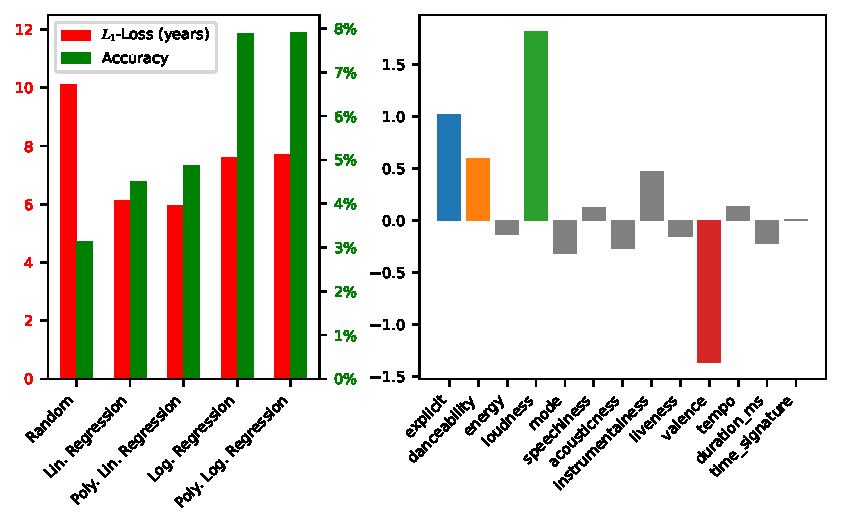
\includegraphics{losses_lincoefs}
  \caption{\emph{Unfair} comparison of the mean absolute error (MAE) in years (lower is better) and accuracies (higher is better) of the Predictors (left) and the coefficients of the linear regression model (right).}
  \label{fig:losses_lincoefs}
\end{figure}
\subsection{Models}

The left side of Figure~\ref{fig:losses_lincoefs} shows some evaluation metrics of the models, performed on the test set. 
Both of these comparisons are hardly fair, as the models are optimized on very different things, but the comparison to randomly generated numbers shows us, that none of them are particularly good. Considering the complicated nature of the data, however, this is not very surprising, as the model has to deal with countless outliers and the fact that it only has very few very basic features at hand.
Another thing that is clearly visible, is that the models using the polynomial feature vector barely outperform their linear counterparts.

\begin{figure}[t]
  \centering
  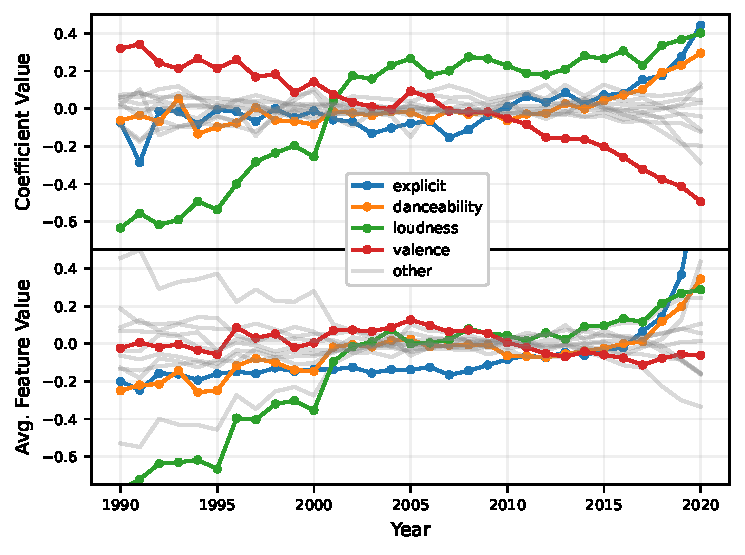
\includegraphics{coefs_avg}
  \caption{The coefficient for each year produced by the logistic regression model (top) and the average value of the features in each year (bottom). The colored lines represent the coefficients with the highest values in many years and their corresponding features. This makes them more important for the logistic regression predictor than the remaining features (grey).} 
  \label{fig:coefs_avg}
\end{figure}
\subsection{Coefficients}

We now try to interpret the coefficients of the models we have build. Because it is much more complicated, while not providing significantly better performance, we throw out the polynomial feature vector. Looking at the coefficients of the linear regression model can already tell us some things about the development of the corresponding features over time. Figure~\ref{fig:losses_lincoefs} shows these coefficients. For example we can now say, that a higher value of the feature \emph{"loudness"} results in a higher output of the model. Thus, in reverse this means that the model assumes songs that have been released later to have a higher \emph{"loudness"}-value.

The logistic regression model gives us a coefficient for each feature in every year, as the output of the model is now a vector of probabilities for the song being released in each year (or alternatively simply the year with the highest probability). These coefficients can be seen in the top part of Figure~\ref{fig:coefs_avg}. While the relationship is not linear, a high coefficient still means a high probability given a high feature value. By looking at this plot, we could for example interpret that, according to the model, in the early 90s many songs have a high valence (i.e. sound happier), while recently more songs with a low valence were released.
Most of the coefficients are very close to 0 in all years and only a few, which can be assumed to have high predictive value, have high and low values in different years. 
In contrast to that, the mean value per year of the features, displayed in the bottom of Figure~\ref{fig:coefs_avg}, does not show the same features with high predictive values standing out at all. Additionally, some curves, like the \emph{valence} coefficient show trends, that the mean does not.


\section{Conclusion}

From the resulting coefficients, one could make the conclusion that in the 90s many songs were relatively happy and quiet, while in the late 2010s the music is much sadder, louder with more songs being rated explicit. While this may or may not be true, the experiment conducted here does not support assumptions like that.

Between the arbitrary features the dataset that we know very little about, and the predictions of the models not being very good. We can not confidently conclude anything about the development of music.

\bibliography{references} 

\end{document}
